\documentclass[11pt]{article}
\usepackage{graphics,epsfig,amsmath,amssymb}
\usepackage{epsf}
\usepackage{boxedminipage}
\usepackage{fullpage}
\usepackage{fancyheadings}
\usepackage{times}
\usepackage{amsmath}
\usepackage{ifthen}
\usepackage{pseudocode}
\usepackage{array}
\usepackage{psfrag}
\usepackage{color}
\pagestyle{fancy}

\setlength{\topmargin}{.2in}
\setlength{\parindent}{0in}
\setlength{\parskip}{.15in}
\setlength{\footskip}{0.1in}

\newcounter{pctr}
\stepcounter{pctr}

\newcounter{partctr}

\newcommand{\ie}{{\em i.e.}}
\newcommand{\eg}{{\em e.g.}}

\newcommand{\ch}{\item {\bf True~~/~~False~~}}
\newcommand{\tfnote}{\probnote{Circle True or False for each choice.}}
\newcommand{\allapply}{\probnote{Circle ALL that apply}}
\newcommand{\bestanswer}{\probnote{Circle the BEST answer}}
\newcommand{\ansbelow}{\probnote{Answer legibly in the space below.}}

\renewcommand{\thesection}{{\bf\Roman{section}}}
\renewcommand{\theenumi}{{\bf\Alph{enumi}.}}
\renewcommand{\labelenumi}{{\bf\Alph{enumi}.}}

\newcommand{\setversion}[1]{\def\version{#1}}
\setversion{exam}

\ifthenelse{\equal{\version}{answers}}{
    \newcommand{\sols}[1]{{\color{blue} #1}}
} {
    \newcommand{\sols}[1]{}
}


\newcounter{answer}
\newenvironment{answer}[1][\relax]{\refstepcounter{answer}\begin{list}%
 {}{\leftmargin 0pt\rightmargin 0pt\labelsep 3pt\parsep 0pt%
 \setlength{\listparindent}{\parindent}}
    \item {\bf Answer \theanswer #1}\
    }{\hspace*{\fill}$\blacksquare$\end{list}} 



% uses these macros to delimit problems
\newcommand\prob[1]%
  {\begin{itemize}\item[]%
   \vspace{.2in}{\bf\thepctr. ~[#1~ points]:}\stepcounter{pctr}}
\newcommand\eprob{\end{itemize}}
\newcommand\probnote[1]%
  {\\\begin{tabular}{cr} \hspace{3in} & {\bf (#1)} \\ \end{tabular}}

% headers/footers
\lhead[\fancyplain{}{\bf Page \thepage ~of \pageref{lastpage}}]%
      {COS 432 Fall 2016, Midterm II}
\lfoot[{\bf Initials: }]%
      {{\bf Initials: }}
\rhead[COS 432 Fall 2016, Midterm II]%
      {\fancyplain{}{\bf Page \thepage ~of \pageref{lastpage}}}
\cfoot{}
\setlength{\headrulewidth}{0in}
\setlength{\headsep}{.3in}

 % Compact itemize and enumerate.  Note that they use the same counters and
% symbols as the usual itemize and enumerate environments.
\def\compactify{\itemsep=0pt \topsep=0pt \partopsep=0pt \parsep=0pt}
\let\latexusecounter=\usecounter
\newenvironment{CompactItemize}
  {\def\usecounter{\compactify\latexusecounter}
   \begin{itemize}}
  {\end{itemize}\let\usecounter=\latexusecounter}
\newenvironment{CompactEnumerate}
  {\def\usecounter{\compactify\latexusecounter}
   \begin{enumerate}}
  {\end{enumerate}\let\usecounter=\latexusecounter}

\begin{document}
\cfoot{}
\pagestyle{empty}
\begin{center}
\begin{tabular}{lr}
\resizebox{1.5in}{!}{
\includegraphics{princeton}}
&
\parbox{4in}{
\vspace*{-0.2in}
   {\Large\sf Department of Computer Science} \\ 
}
%
\end{tabular}
\end{center}

\begin{center}
{\LARGE{\bf Midterm II}} \\
\vspace{.15in}
{\Large{\bf COS 432: Information Security: Fall 2016}} \\
\vspace{.2in}

% this is the box on the first page with overall quiz information
\begin{boxedminipage}[h]{6in}
  There are \underline{11 questions} and \underline{\pageref{lastpage}
    pages} in this quiz booklet (including this page). {\bf There are
    160 total points.}  Answer each question according to the
  instructions given.  You have {\bf 80 minutes} to answer the
  questions.

\vspace{.1in} 
If you find a question ambiguous, write down any
assumptions you make.  {\bf Be neat and legible.}  If we can't
understand your answer, we can't give you credit!  
%There are three pretty
%challenging questions (clearly marked); you may want to look through the
%whole quiz and save those for last.

\vspace*{.1in} {\bf Lifeline:} For {\em one} part (\ie, capital alphabetic
letter) of any question, you can write ``SKIP''. For that portion of the
question, you will receive full credit (\ie, 10 points).

\vspace{.1in} 
Use the empty sides of this booklet if you need scratch space.  You
may also use them for answers, although you shouldn't need to.  {\em If you
do use the blank sides for answers, make sure to clearly say so!}

\vspace{.1in} 
{\bf Note: Write your name in the space below AND your initials at the bottom of each
page of this booklet.}

\begin{center}{\bf THIS IS AN ``OPEN NOTES'' QUIZ.\\
ONE TWO-SIDED LETTER-SIZED NOTE SHEET AND THE LECTURE NOTES HANDOUT IS
ALLOWED. \\ 
MAKE SURE YOU'VE READ ALL THE INSTRUCTIONS ABOVE!}
\end{center}
{\em (1)~Initial here to indicate that you've read the instructions: \\ 
(2)~In the space below, write out and sign the Princeton Honor Code pledge before 
turning in the exam: ``I pledge my honor that I have not violated the Honor Code during this examination.'' }
\vspace{0.5in}
\\


\if 0
\vspace{.05in} 
The last page has a course questionnaire, {\em which you can
answer outside of the allotted time}.  Rip the last page off of your
quiz for five bonus points.  Turn it in anonymously if you like (feel
free to fill it out after the quiz and give it to a TA, or take it with
you).  
You
won't get the five points if you don't tear off the page (this is to
make certain you've read this far ;).
\fi 

\end{boxedminipage}
\end{center}
\vspace*{0.05in}
\begin{center}
{\it Do not write in the boxes below}
\end{center}

\begin{center}
\begin{tabular}{|l|l|l|l|l|l|l|l|l|} \hline \hline
{\bf 1-3 (xx/30)} & {\bf 4-5 (xx/20)} & {\bf 6-7 (xx/40)} & {\bf 8-9
  (xx/40)} & {\bf 10-11 (xx/30)} & {\bf Total
  (xx/160)}  \\ \hline 
& & & & & \\ 
& & & & & \\ \hline \hline
\end{tabular}
\end{center}

\vspace{.1in}
{\bf\Large{Name:}}

\newpage
\pagestyle{fancy}

\section{Buffer Overflows and Code Injection}

The following questions concern buffer overflows and code injection. 
(Note: Each sub-problem can be answered with a short phrase/explanation. If
you are writing a paragraph or explaining a complicated design, you're
probably spending too much time.

\prob{10}
Recall the {\tt strcpy()} function: 
\\( {\tt char *strcpy(char *dest, const char *src)}: The strcpy() function copies
the string pointed to by src, including the terminating null byte, to the buffer pointed to by dest.)

Why is {\tt strcpy()} vulnerable to a buffer overflow attack? What extra
argument is needed to secure it against buffer overflows?

\sols{
The buffer size is not determined for strcpy so that the adversary can easily create a buffer overflow and overwrite important areas such as return addresses.
}
\eprob
\vspace*{0.5in}

\prob{10}
Pushing to the stack and running user-provided shellcode in Assignment
2 was one example of a code injection attack; a SQL injection attack is another
type of code injection attack. 
{\em In general, what is the vulnerability that code injection attacks typically
exploit? (One sentence/phrase.)} 

\sols{
The user input is interpreted as code not as data.
}
\eprob
\vspace*{0.5in}

\prob{10} What is one protection mechanism to prevent code injection attacks (buffer
overflows or SQL injection)?

\sols{
Data Execution Prevention (DEP). DEP marks areas of memory as either executable
or non-executable (read/write) so that data is not interpreted as code in memory.  
}
\eprob
\vspace*{0.5in}

\if 0
\prob{10} Let's assume now that a protection mechanism against code injection
attacks is in place. Assuming that the attacker can overwrite the stack, is it
possible for the attacker to gain control of the system (\eg, by opening a root
shell).

\sols{
Still vulnerable to code reuse attacks. Redirect the control flow to code that has the desired functionality and it's already there in the code segment. Since the attacker controls the stack, she can define the arguments for the used functions.
}
\eprob

\item Mention and briefly explain a defense that makes any stack smashing attack
harder.

\sols{
  ASLR                                                                                                                                                  
}
\eprob
\fi




\newpage
\section{Web Security}

Much of this problem should be familiar from Assignments 2 and 3. The
code snippets should also be familiar, but be careful, as there are a few small
changes.

\prob{10}
What is a CSRF attack? Explain the purpose of token validation that you learned
from the assignment.

\sols{
    These are the easiest questions. I think the homework for this part is either easy or related to XSS attack. So I just come up a question about definitions. 
}
\eprob
\vspace*{0.5in}

\prob{10} Consider a web server that is running the following PHP code to authenticate
users:
{\footnotesize
\begin{verbatim}
if (isset($_POST[’username’]) and isset($_POST[’password’])) {
    $username = $_POST[’username’];
    $password = $_POST[’password’];
    $sql_s = "SELECT * FROM users WHERE password='$password' and username='$username'";
    $rs = mysql_query($sql_s);
    if (mysql_num_rows($rs) > 0) {
        echo "Login successful!";
    } else {
        echo "Incorrect username or password";
    }
}
\end{verbatim}
}
Write an input pair (username, password) that bypasses authentication procedures
and logs in as a user named `admin'. Briefly explain your answer. (Hint: `and' has
a higher precedence than `or')
\eprob

\sols{
	username = admin; password = ' or ''='; It is almost the same as the homework but I simply change the order of username and password. 
}

\if 0
\prob{10} Consider a web server that uses the following PHP code to authenticate 
users:
{\footnotesize
\begin{verbatim}
if (isset($_POST[’username’]) and isset($_POST[’password’])) {
    $username = $_POST[’username’];
    $password = md5($_POST[’password’], false);
    $sql_s = "SELECT * FROM users WHERE username=’$username’ and pw=’$password’";
    $rs = mysql_query($sql_s);
    if (mysql_num_rows($rs) > 0) {
        echo "Login successful!";
    } else {
        echo "Incorrect username or password";
    }
}
\end{verbatim}
}

Note that this code uses {\tt false} as the second parameter of the {\tt
md5()} function, which cases the function to return the hash as a $32$-character
hexadecimal number in string. {\bf Is this code secure against any SQL
injection?} (Yes or no.) If so, explain why. If not, provide an input pair
(username, password) that bypasses authentication procedures by logging in as
a user named `admin'. In addition, suggest a solution to fix this code and
protect against any SQL injection if you think this code is vulnerable. (Hint:
\#, -- are two possible comment characters in MySQL)

\sols{
	The answer is NO. Let username = admin';\#  and password be an empty string. Prepared statement or escaping username (and password). 
}
\eprob

\prob{10}  Recall that for the XSS attack assignment, you were asked to
demonstrate XSS attacks against Bungle’s search box, which does not properly
filter search terms before echoing them to the results page. Your goal was to
construct a URL that, if loaded in the victim’s browser, correctly executes
the payload which required persistence as one of the requirements.

Provide a step-by-step explanation of how how you made your payload persist
when a user logged into Bungle with his account. (You are not required to
explain how to deal with the backward/forward buttons.) {\em Your answer should
be no longer than about five steps; one short phrase for each step is sufficient.}

\sols{
	\begin{itemize}
	\item  remove original functionality of login button
	\item  bind login button with a new onclick event handler
	\item  read user input using jQuery/javascript function from username and userpass fields\\
	\item  using \$.ajax or other equivalent function to submit a POST request\\
	\item  reload the page by calling function equivalent to proxy() from framework code
\end{itemize}
}

\eprob
\fi

\newpage
\section{Network Firewalls}

You are hired as the new network security advisor of Legitimate
Software Inc, a company that distributes decent software products. 

Currently, Legitimate Software products can be downloaded from the company
home page LSI.com, which is hosted on a HTTP web server within the company.
Programmers of Legitimate Software regularly update their products, and upload
the new software patches from company workstations to the web server.

\prob{20}
The company tech lead asks you to set up a firewall between company
machines (including the web server and workstations used by programmers) and
the external Internet, only allowing connections originating from a internal
host. 
\begin{enumerate}
\item List two different attacks (malicious activities) this firewall could
prevent. 
\item Describe a {\em legitimate} use of the company's
network that this firewall setup would also prevent.
\end{enumerate}

\sols{
  Attacks that could be prevented: Listing all hosts on the company's network (via ping); Logging onto the workstations using stolen passwords; Connecting to company databases from the Internet; 
  Legitimate uses that are also prevented: Download products from company's website from the Internet; Working from home (access workstations from the Internet, with correct credentials);
}
\eprob

\newpage
\prob{20} The tech lead asks you to fix the company's firewall configuration
to address the
shortcoming from
the previous question. Create a firewall
{\bf (A)~topology}; and {\bf (B) policies} that satisfy the following requirements:

\begin{itemize}
\item Customers
can visit the company's web site to download new software through HTTP (port
80), from anywhere on earth. 
\item Programmers in the company can upload files to
the web server through SSH (port 22), only when they are using the company
workstations. 
\item No network connections can be made to the company
workstations, unless the connection originate from one of the workstations. 
\item
Programmers can access the Internet (\eg, visit http://stackoverflow.com) on
their workstations. (Hint: divide the machines to multiple groups and set up
multiple firewalls in between.)
\end{itemize}
{\em Hint:} You will need more than one firewall. It will likely be faster to
write down your answer as a {\em picture} that shows the Internet, the company
web server, and the rest of the company network, as well as where you would
place firewalls and what policies should exist on each of them.

\sols{
  Internet <-> (||firewall1||) <-> web server <-> (||firewall2||) <-> workstations
  firewall1 minimum policies: drop connections from Internet, unless their destination is web server port 80
  firewall2 minimum policies: drop all connections from outside. drop connections from inside, except HTTP traffic to stackoverflow.com and SSH traffic to the web server
}
\eprob


\if 0
\prob{10} The network security of Legitimate Software is greatly enhanced by your
new firewall policy. However, a smart hacker managed to break into the
web server and replaced the software patches with his own malware. 

How would you prevent the illegitimate patches to be applied to Legitimate
products already installed on users' computers? You can assume that before the
attack, everything on users' computers are authentic, Legitimate products.
({\em Hint:} recall what you have learned about digital signatures and public
key infrastructures.)

\sols{
  All Legitimate products should only accept patches with digital signatures (certificates) created with company's private key (assume that this private key is not compromised). There's two possible authentication schemes: ship the software with company's public key, or register company's key with well know Certificate Authority.
}
\eprob
\fi
\newpage
\section{Denial of Service Attacks}

Suppose you operate a web site and would like to make your web site resilient to denial
of service (DoS) attacks (both conventional denial of service attacks, as well as
distributed DoS attacks).

Recall that many denial of service attacks are based on the principle of
asymmetry: without expending many resources, an attacker can cause the victim
to expend many more resources. In this question, we'll review various ways
asymmetry show up in DoS attacks, as well as various mechanisms you might use
to defend against them. Some of these techniques we have discussed in class.
Others may be new, but you should be able to reason through the attack and
defenses based on what we've taught you.

\prob{20} 
You notice that your
web server suddenly receives a flood of TCP SYN packets from many distinct IP
addresses. You realize that you forgot to enable TCP SYN cookies. 

\begin{enumerate}
\item Describe
what might happen to your server without TCP SYN cookies enabled. 
\item Describe why enabling TCP SYN cookies will help defend against the attack
you are witnessing.
\end{enumerate}
\eprob

\if 0
\newpage
\prob{20} After you enable TCP SYN cookies, you notice that your attacker has begun
launching a DDoS attack from many different IP addresses, whereby each IP address
is sending your web server a legitimate HTTP request. 
\begin{enumerate}
	\item Explain why this attack might be more difficult to detect and mitigate as
	compared to a SYN flood attack.
	\item Companies such as CloudFlare use mechanisms such as CAPTCHAs---images and
	words that are difficult for computers to decipher but easier for humans to read---to
	defend against these kinds of attacks. Briefly describe one advantage to using
	a CAPTCHA to defend against this type of DDoS attack; also describe {\em two} disadvantages
	to using CAPTCHAs (Hint: Think about who or what may not be able to solve CAPTCHAs.
	In case you don't know what a CAPTCHA is, it looks like the figure below.)

	\centering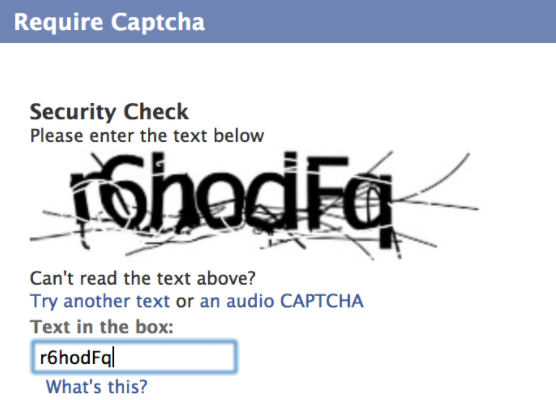
\includegraphics[width=0.3\linewidth]{captcha}
\end{enumerate}
\eprob
\fi

\newpage
\prob{20}
We discussed a large-scale DDoS attack
that was mounted from a collection of insecure Internet-connected DVR cameras on
October 21, 2016. The attack generated about 1.2 terabits per second of attack traffic
and managed to bring down
many web sites (including Twitter, Reddit, and others), {\em without directly sending
traffic to each of these web sites}. 
\begin{enumerate}
	\item Explain how the DDoS attack managed to bring down all of these web sites without
	sending attack traffic to each site directly.
	\item This particular attack did not use reflection or amplification. Suppose,
	however, that each Internet-connected device that participated in this attack had
	been running an open DNS resolver. Describe a modification to the attack that took
	place that could have resulted in an increase in the attack traffic by an order
	of magnitude.
%	\item How might the original attack (which was not a reflection attack) have been
%	prevented? In general, how might a reflection attack be prevented?
\end{enumerate}
\eprob
\newpage
\section{Internet Censorship and Tor}

The following questions concern Tor, and possible attacks against the
anonymity properties that it provides.

\prob{10} 
Recall that each Tor circuit has three relay nodes: a guard, a middle relay,
and an exit node, as shown below. 

\begin{center}
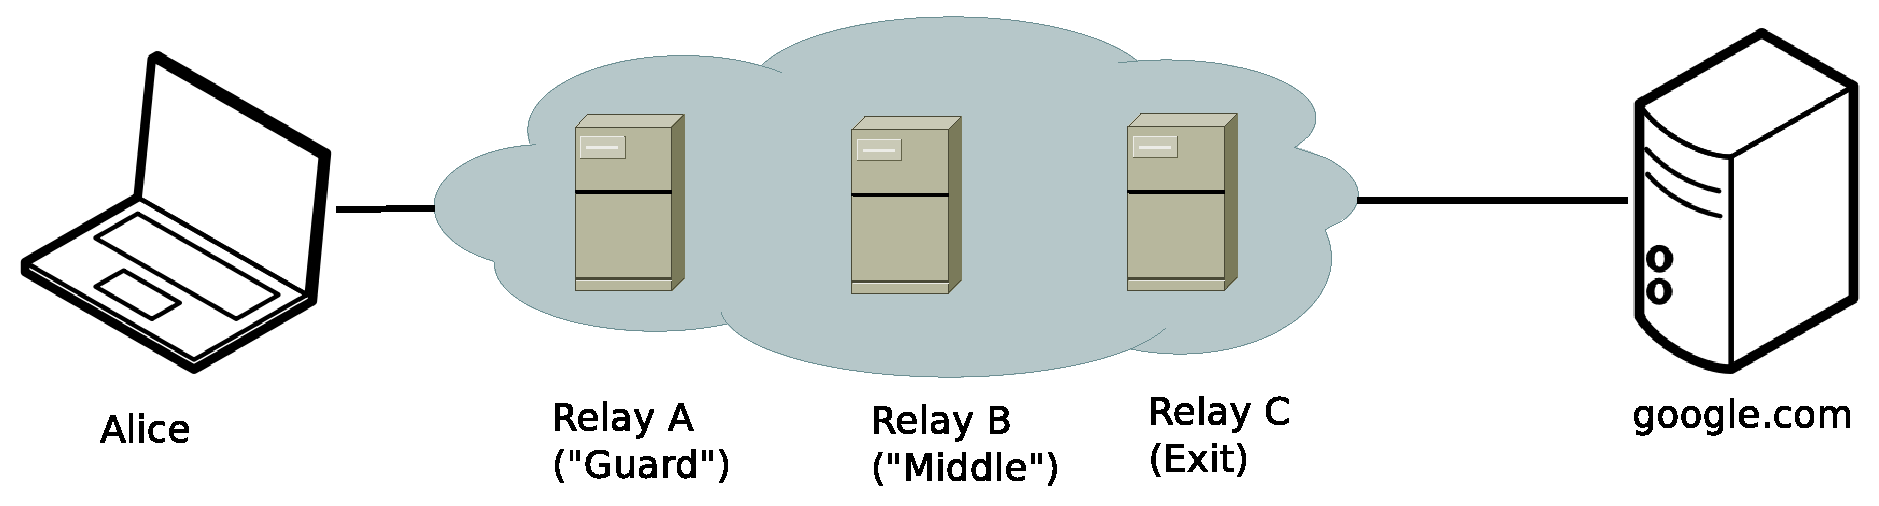
\includegraphics[width=0.65\linewidth]{tor}
\end{center}

Suppose that Alice wants to send a message $m$ to {\tt google.com} through the relays
$A$, $B$, and $C$ below.  {\em Write down the onion encrypted message that Alice's
Tor client would construct.}

Please use the following notation: $\{(A, m)\}_B$ means ``encrypt
$(A,m)$ with $B$'s public key''. $B$ could then decrypt the message $(A,m)$ and
interpret the first part of the tuple as the ``next hop'' $A$, who would receive $m$.  (Hint: Your answer should contain multiple
``onion'' layers of encryption. It should only be one line.)
\eprob

\newpage
\prob{20} 
Recall from lecture that that much of Tor's security depends on
ensuring that no single party has control over multiple nodes, or multiple
parts of the network path between two ends of communication that is taking
place over Tor.  

In class, we talked about Sybil attacks, where an attacker could mount attacks
by controlling multiple {\em relays} in the Tor circuit. This question asks a
related, but slightly different question: What is possible if an attacker can
observe traffic at multiple {\em network observation points} along a path
between two parties communicating over Tor.

Suppose that Alice is a Comcast subscriber and uses Tor to connect to {\tt
google.com} and that her Tor client chooses a circuit with an exit relay that is
{\em also in the Comcast network}.

\begin{enumerate} 
	\item How might Comcast determine be able to determine that Alice is communicating
	with {\tt google.com}? How might it be able to determine the {\em contents}
	of the communication between Alice and {\tt google.com}? 

\item What is a possible defense against the possible attack(s) you
identified in the previous part of the question?
\end{enumerate}

\eprob

\label{lastpage}
\end{document}
i